%\textbf{FIXME: ReRecoed data are used but additional e-scale and smearing corrections NOT yet available and thus NOT yet applied}
Referred to \cite{CMS-PAS-HIG-19-001}.
%Electrons in data are corrected for features in ECAL energy scale
%in bins of $\pt$ and $\left| \eta \right|$. Corrections are calculated
%on a $\cPZ \to \Pe\Pe$ sample to align the dielectron 
%mass spectrum in the data to that in the MC, and to
%minimize its width.
%
%The $\cPZ \to \Pe\Pe$ mass resolution in Monte Carlo is made to match
%data by applying a pseudorandom Gaussian smearing to electron energies,
%with Gaussian parameters varying in bins of $\pt$ and $\left| \eta \right|$.
%This has the effect of convoluting the electron energy spectrum with a
%Gaussian.
%
%The electron energy scale is measured in data by fitting a Crystall-ball function to the di-electron mass spectrum around the Z peak in the $Z\rightarrow \Pe \Pe$ control region. The energy scale for the 2016, 2017 and 2018 dataset are shown in Fig.~\ref{fig:ele_energy_scaleA},~\ref{fig:ele_energy_scaleB},~\ref{fig:ele_energy_scaleC} (a), respectively, and decently agrees with the MC with the preliminary corrections released so far by EGAMMA POG. % for Moriond. % even without any corrections available at the moment. 
%
%\begin{figure}[!htb]
%\vspace*{0.3cm}
%\begin{center}
%\subfigure [] {\resizebox{8cm}{!}{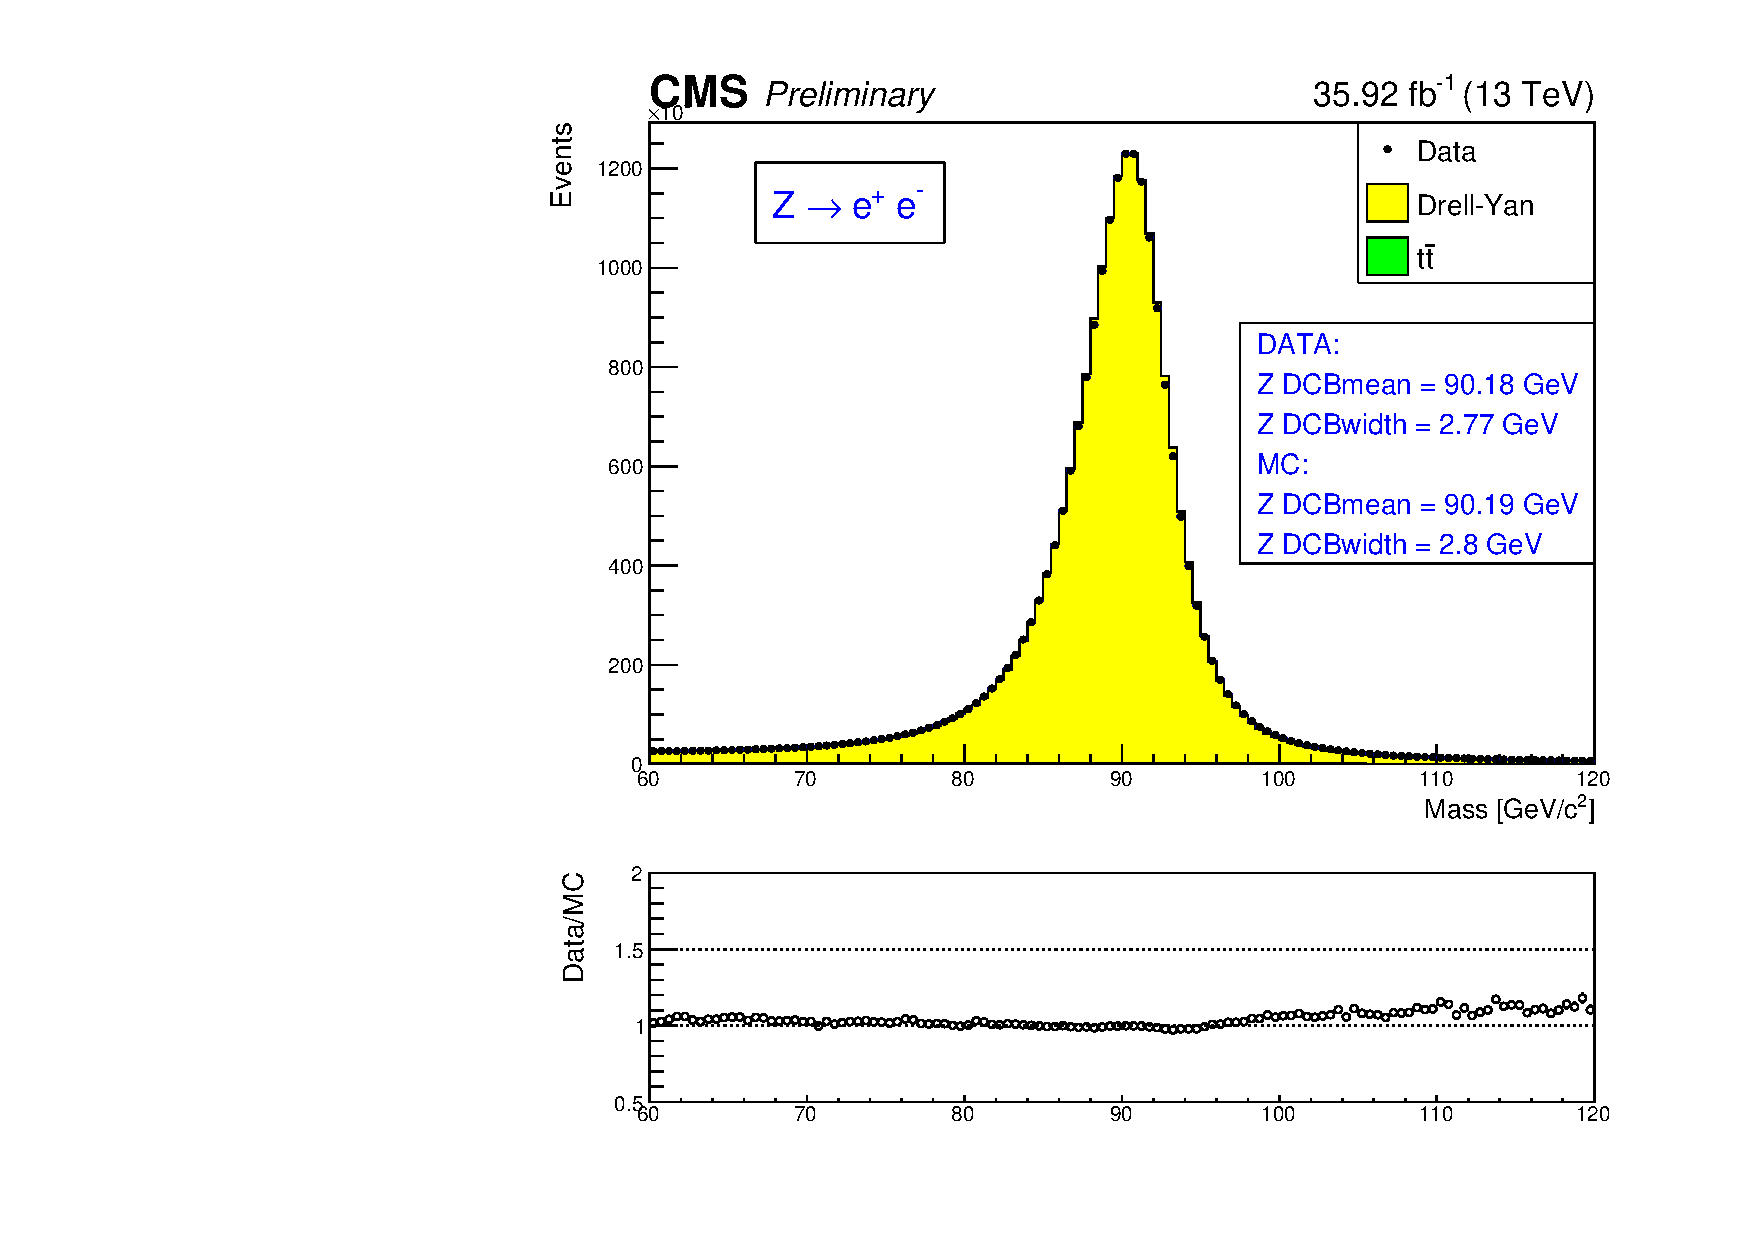
\includegraphics{Figures/Electrons/2016_ZMass_ele.pdf}}}
%\subfigure [] {\resizebox{8cm}{!}{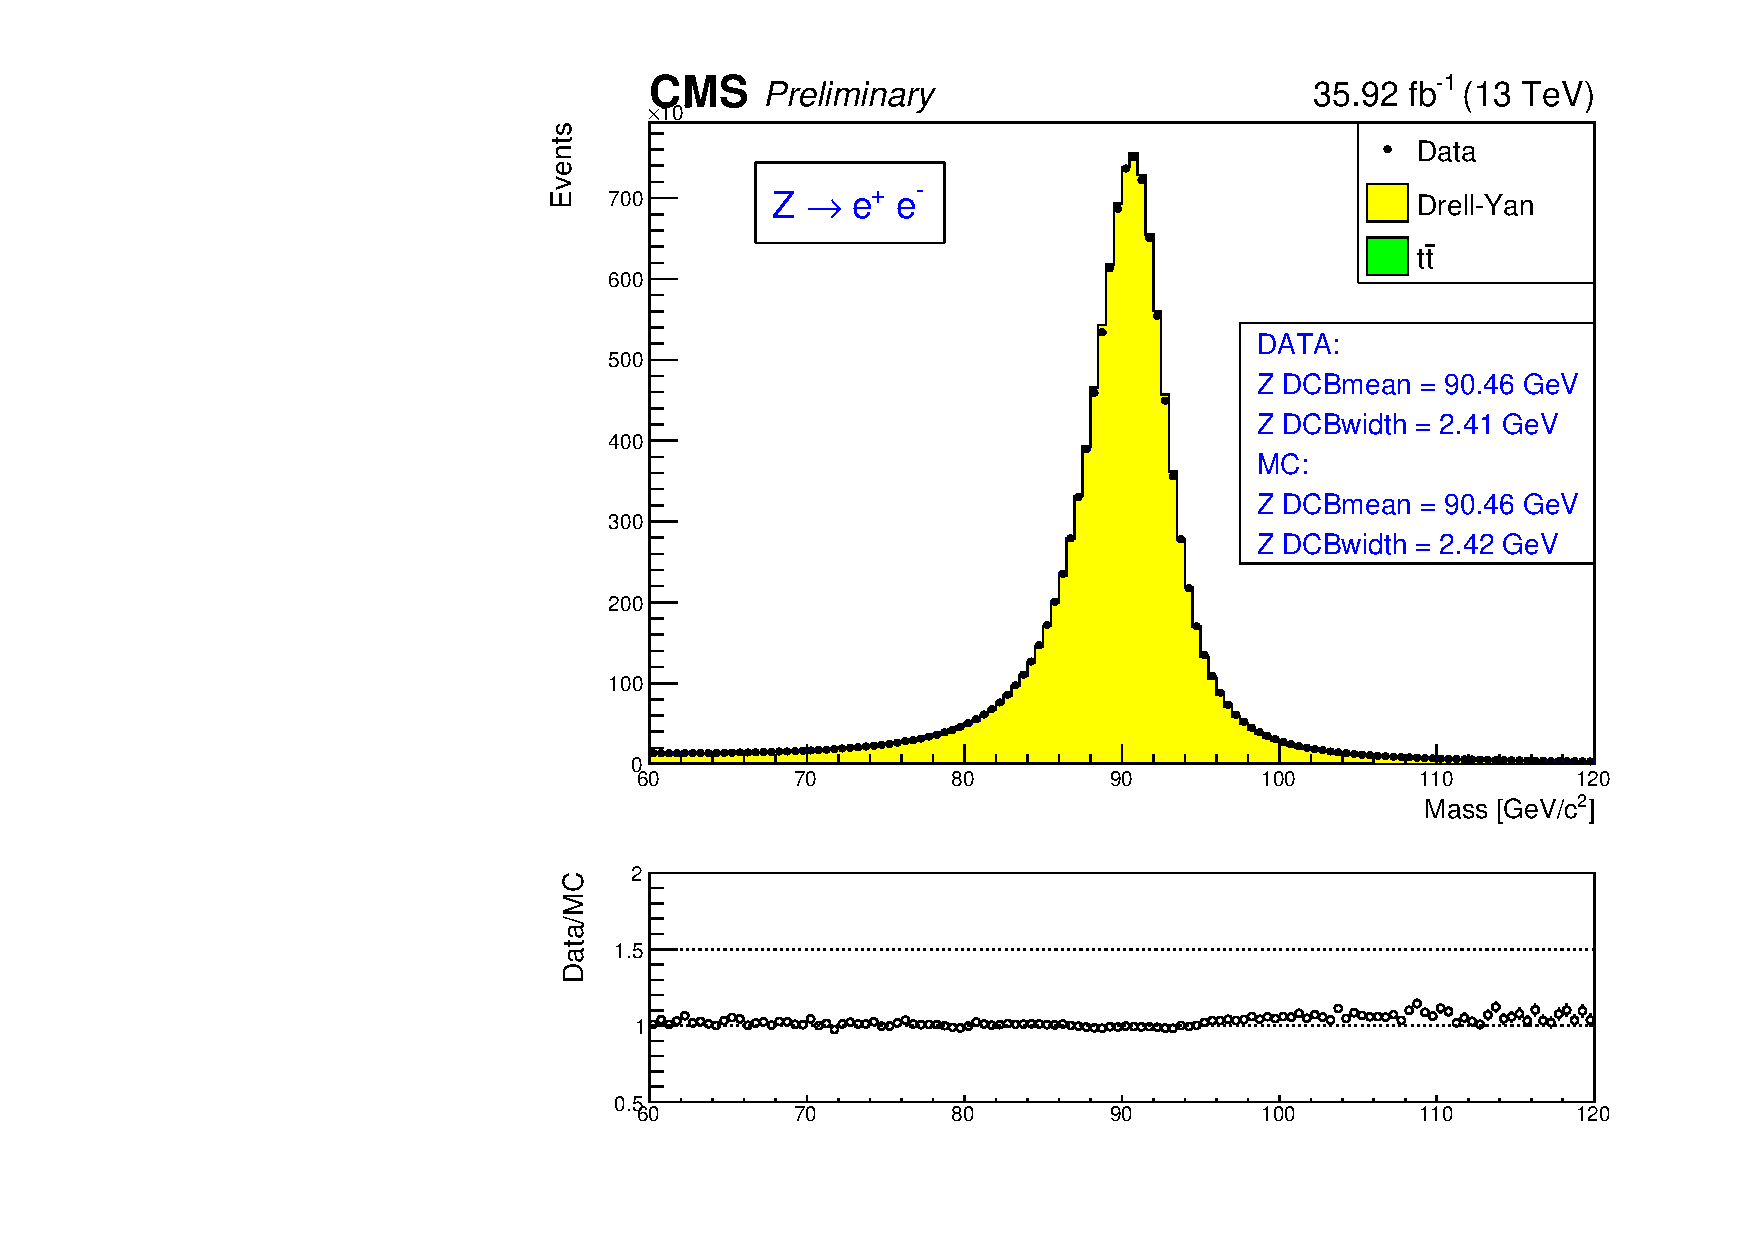
\includegraphics{Figures/Electrons/2016_ZMass_ele_EBEB.pdf}}} \\
%\subfigure [] {\resizebox{8cm}{!}{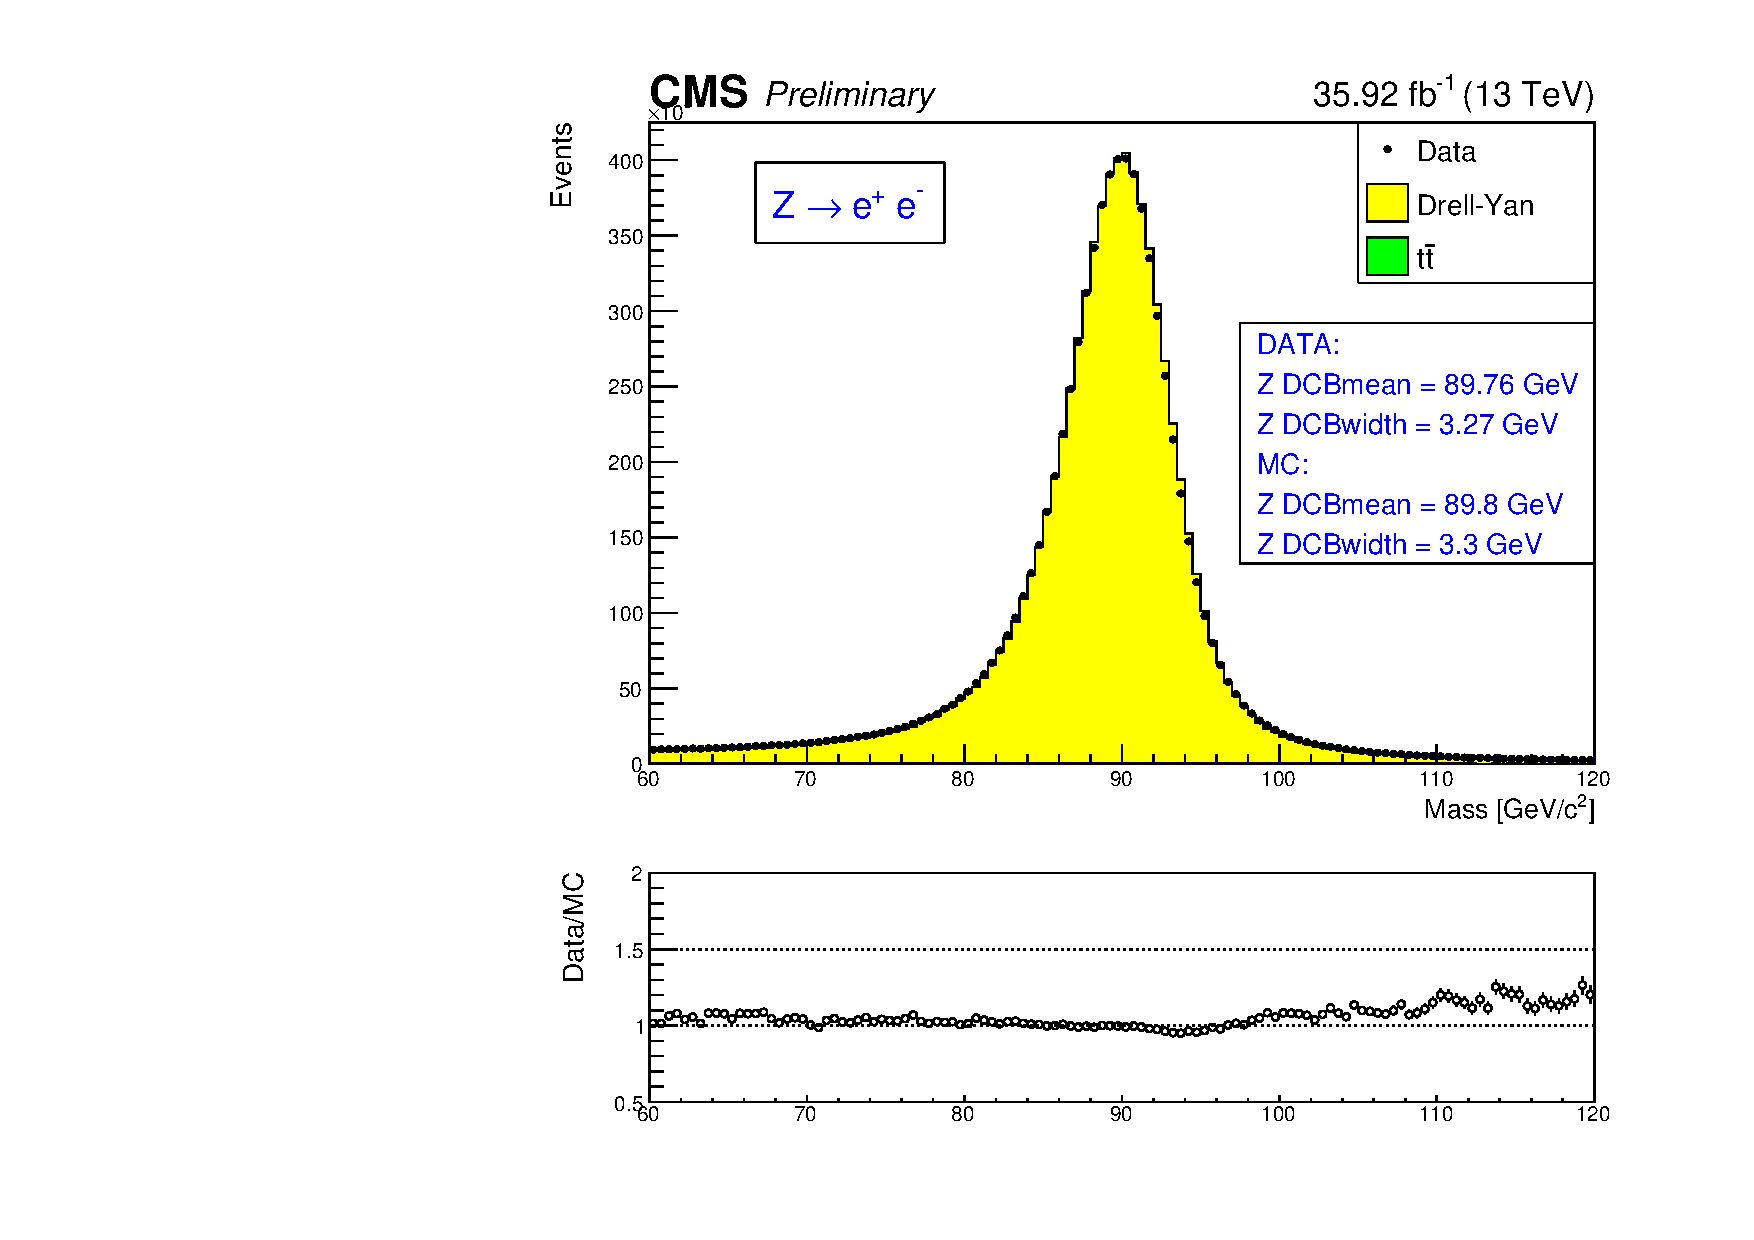
\includegraphics{Figures/Electrons/2016_ZMass_ele_EBEE.pdf}}}
%\subfigure [] {\resizebox{8cm}{!}{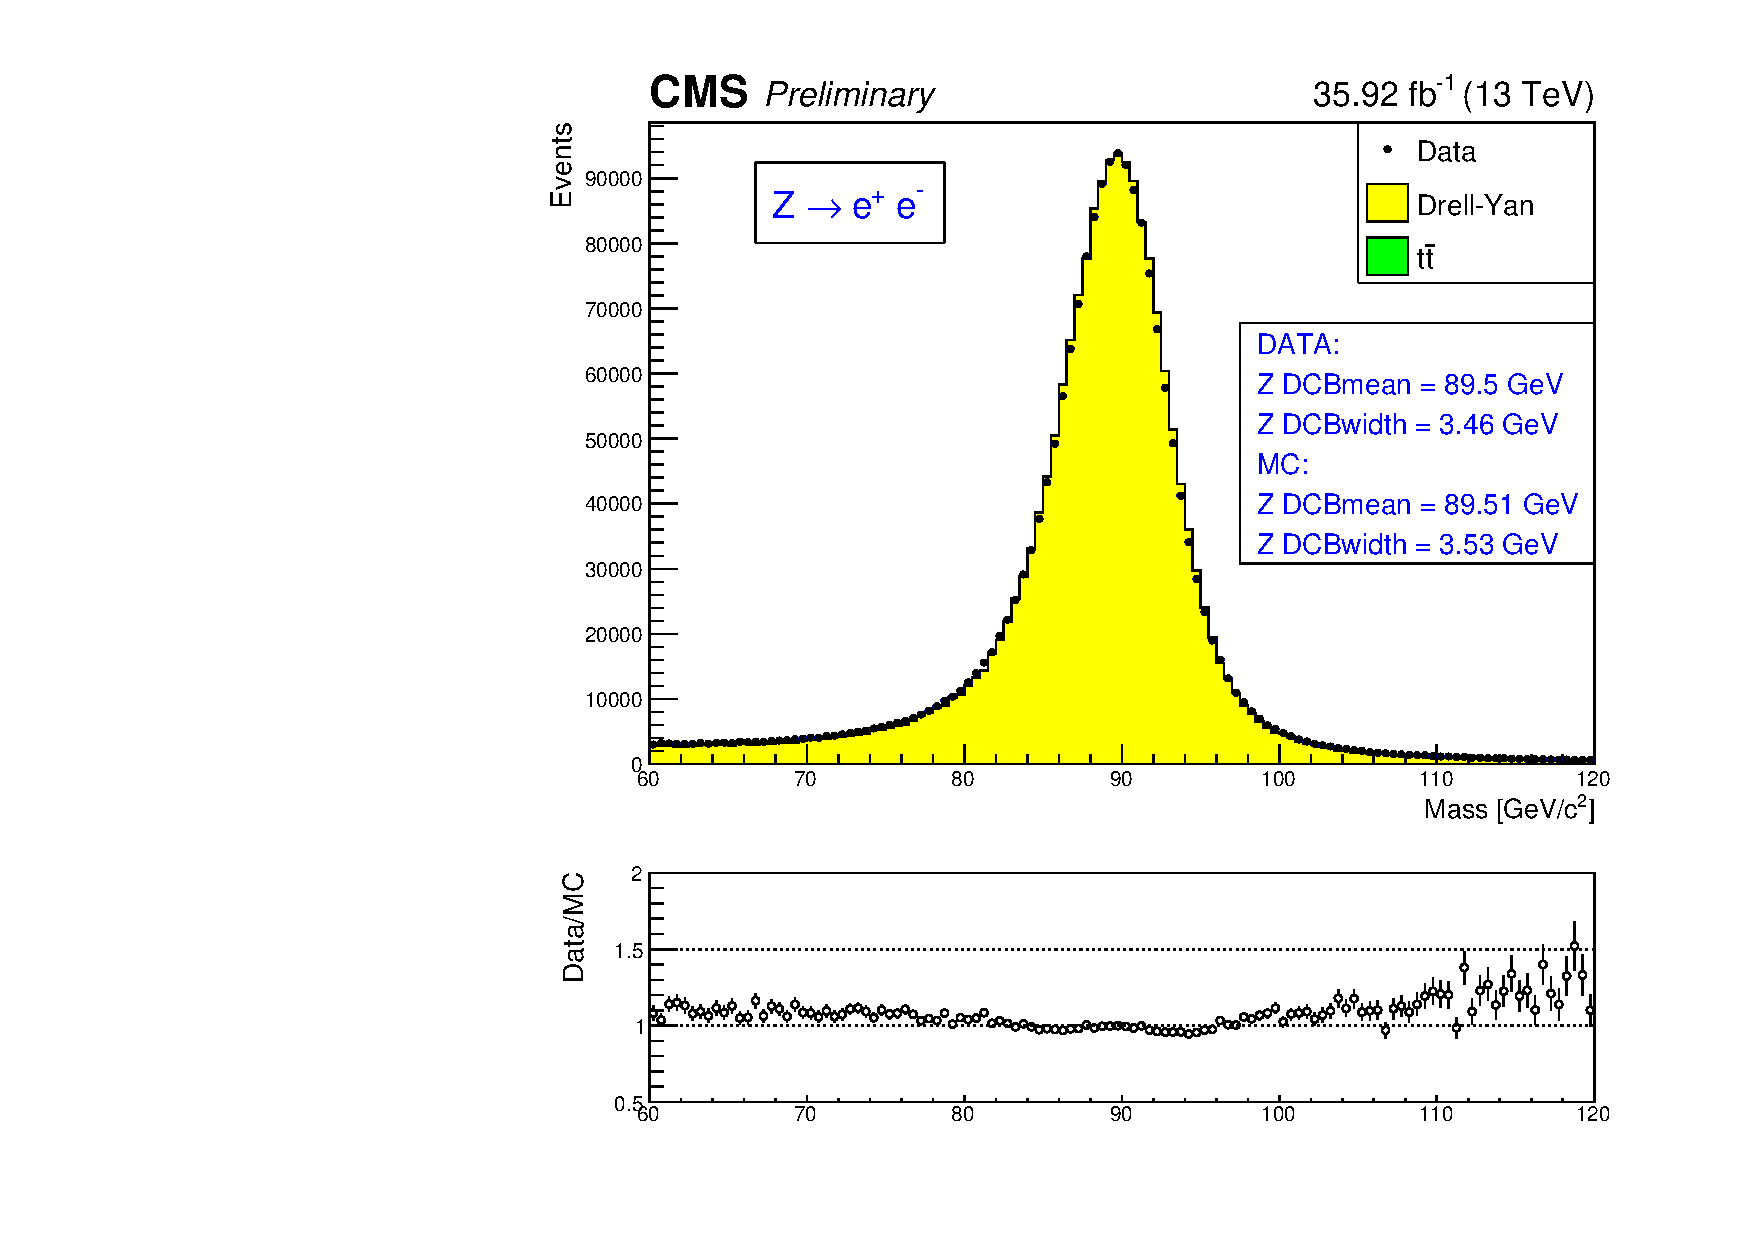
\includegraphics{Figures/Electrons/2016_ZMass_ele_EEEE.pdf}}} \\
%\end{center}
%\caption{
%(a): electron energy scale measured in the $Z\rightarrow \Pe \Pe$ control region for all electrons, for both electrons in the barrel (b), for one electron in the barrel, one in the endcaps (c) and for both electrons in the endcaps (d), for 2016 data.
%The results of the Crystall-ball fit are reported in the figures.
%%\textbf{FIXME: e-scale and smearing corrections NOT yet available and thus NOT yet applied} 
%}
%\label{fig:ele_energy_scaleA}
%\end{figure}
%
%\begin{figure}[!htb]
%\vspace*{0.3cm}
%\begin{center}
%\subfigure [] {\resizebox{8cm}{!}{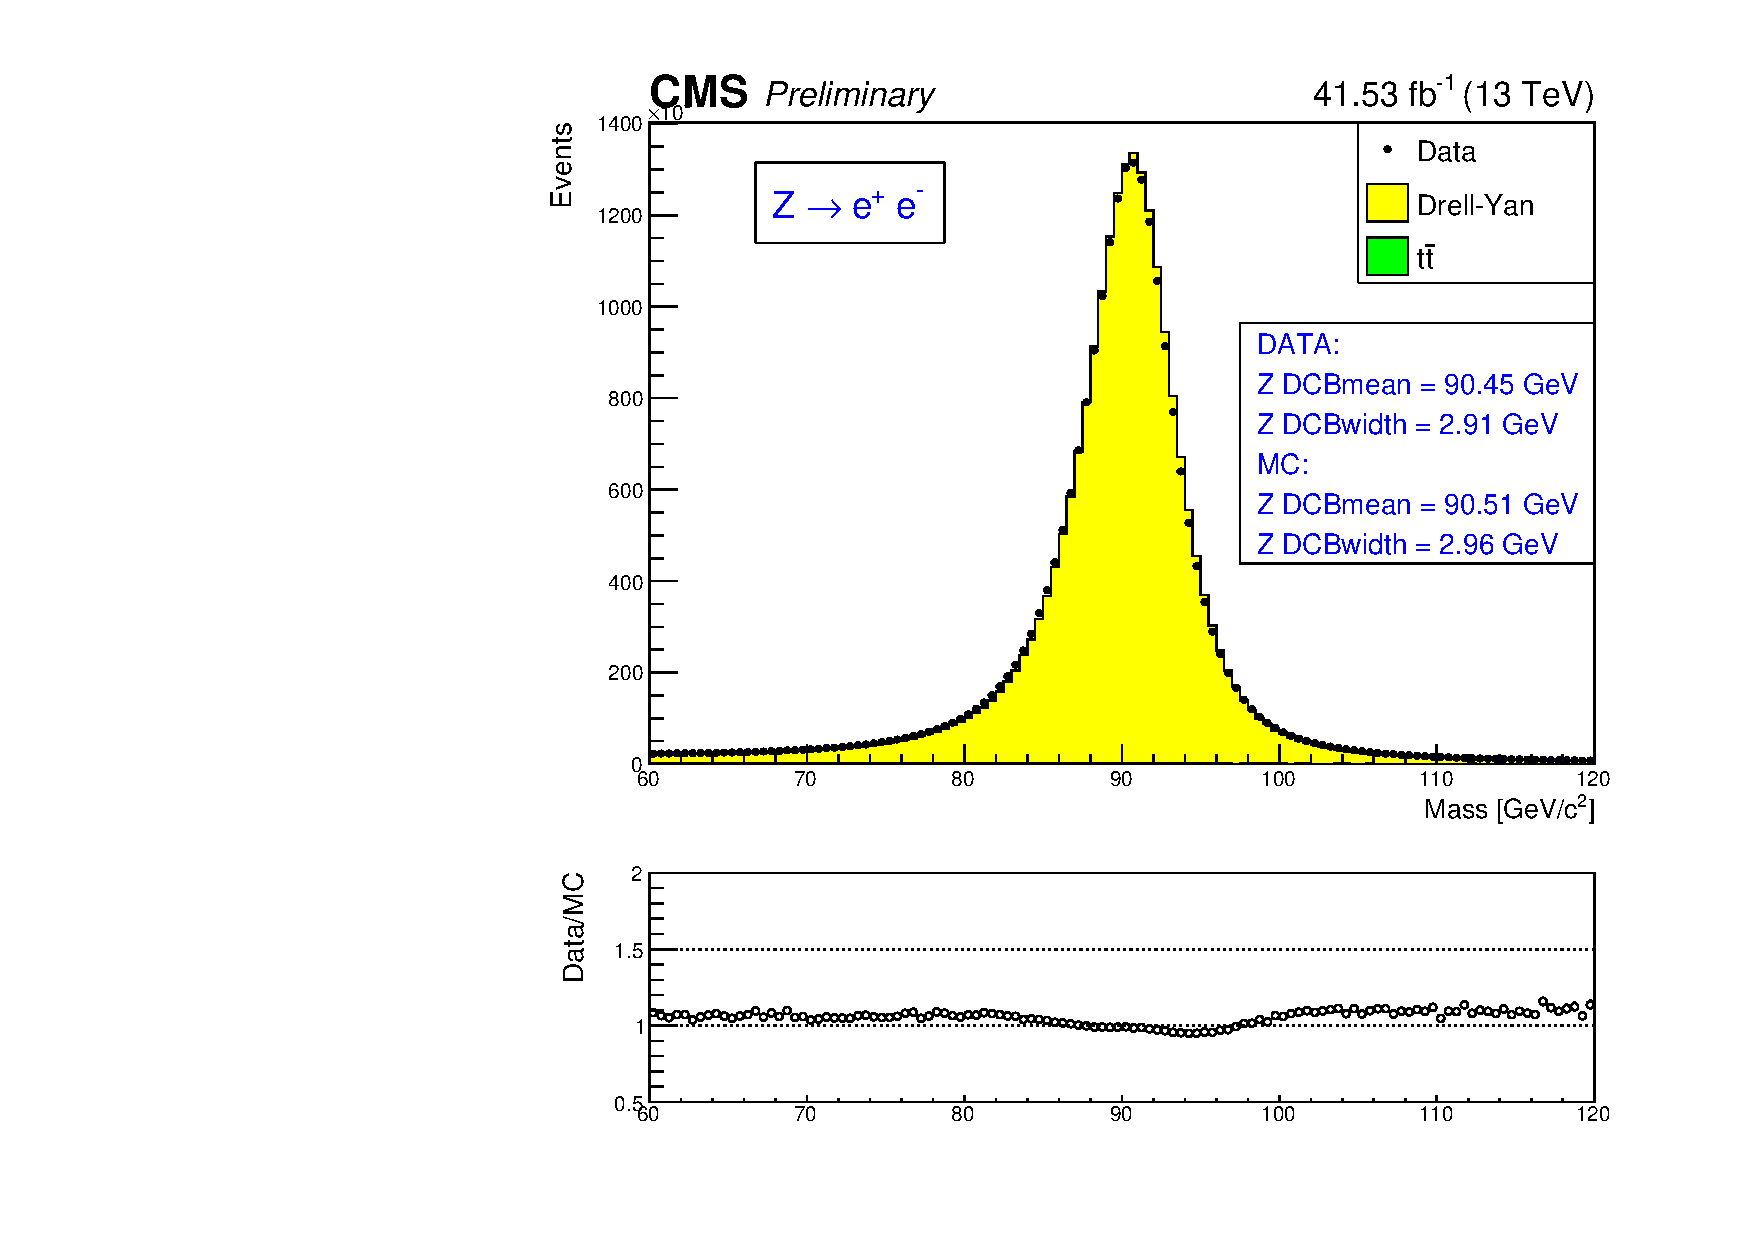
\includegraphics{Figures/Electrons/2017_ZMass_ele.pdf}}}
%\subfigure [] {\resizebox{8cm}{!}{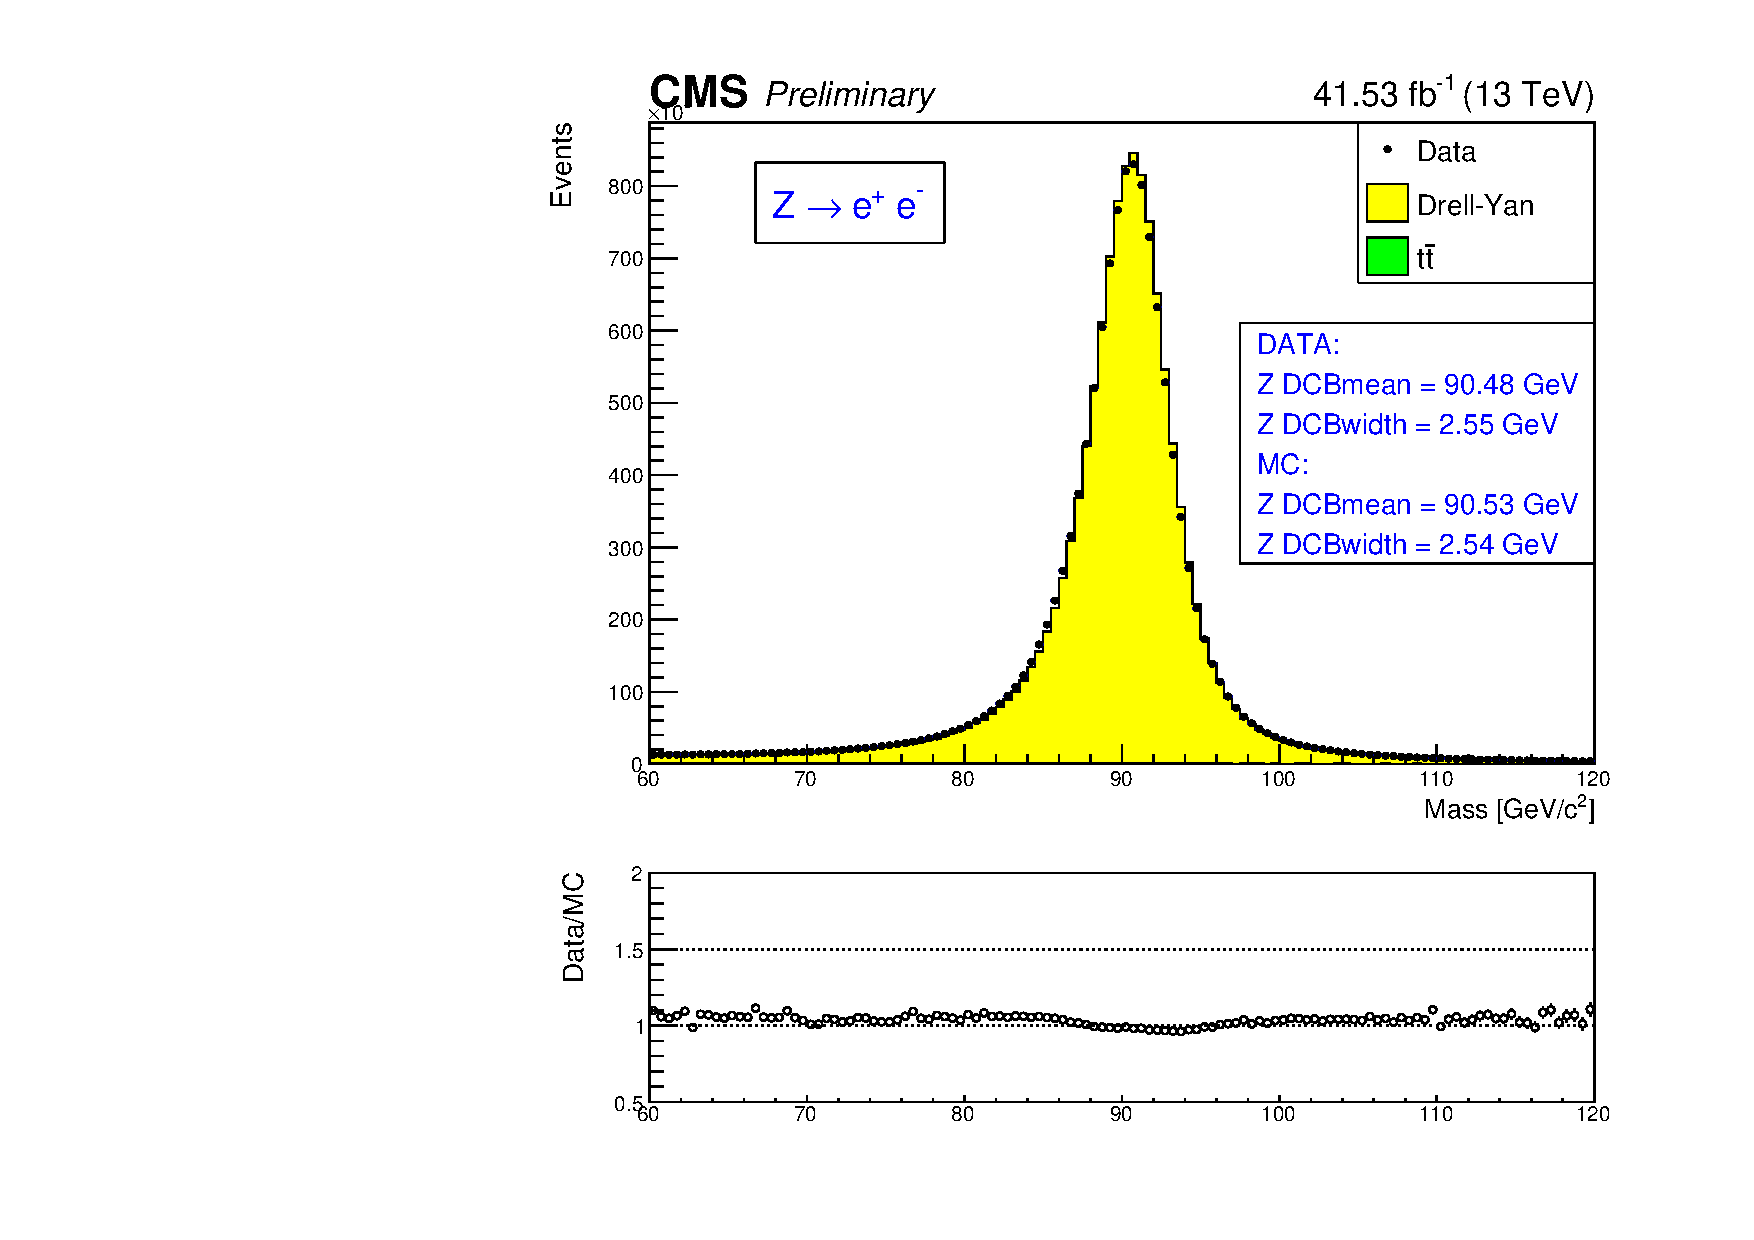
\includegraphics{Figures/Electrons/2017_ZMass_ele_EBEB.pdf}}} \\
%\subfigure [] {\resizebox{8cm}{!}{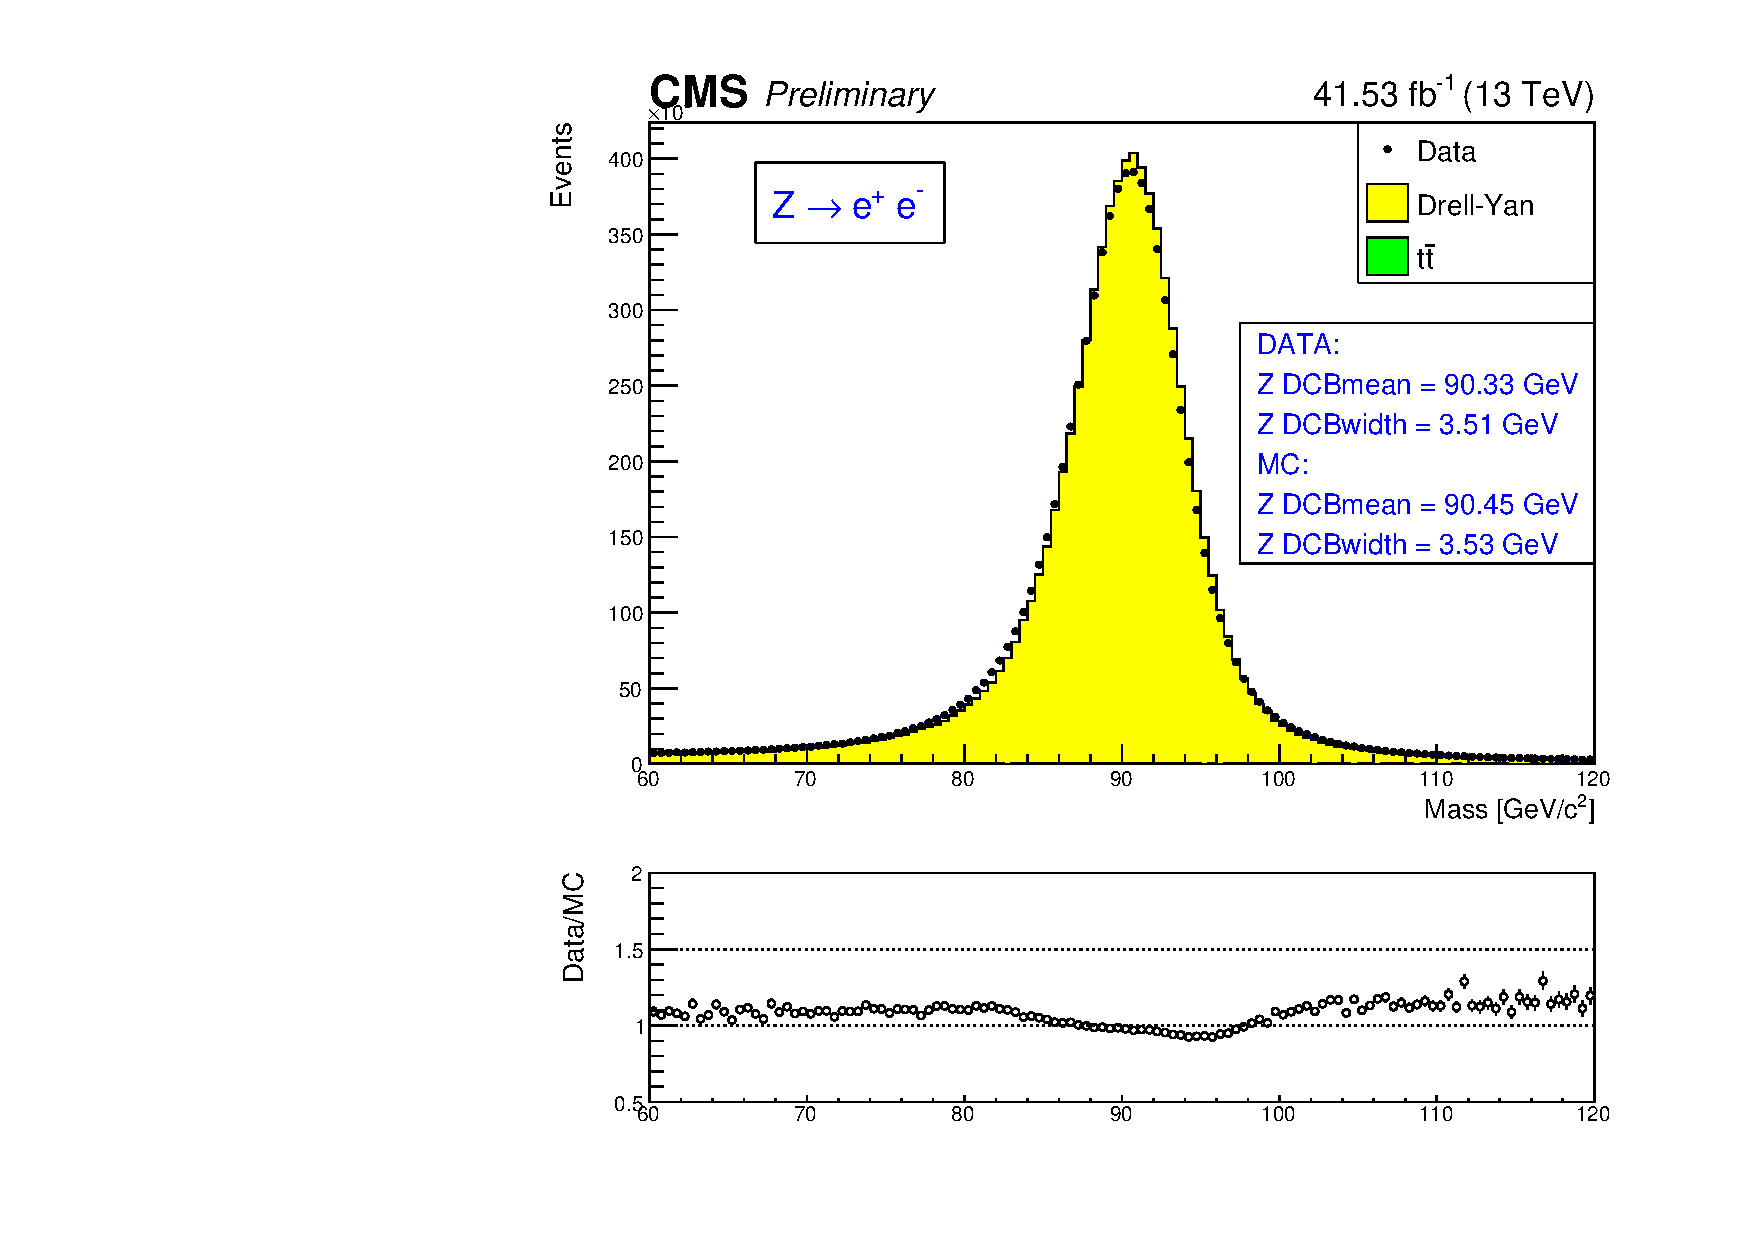
\includegraphics{Figures/Electrons/2017_ZMass_ele_EBEE.pdf}}}
%\subfigure [] {\resizebox{8cm}{!}{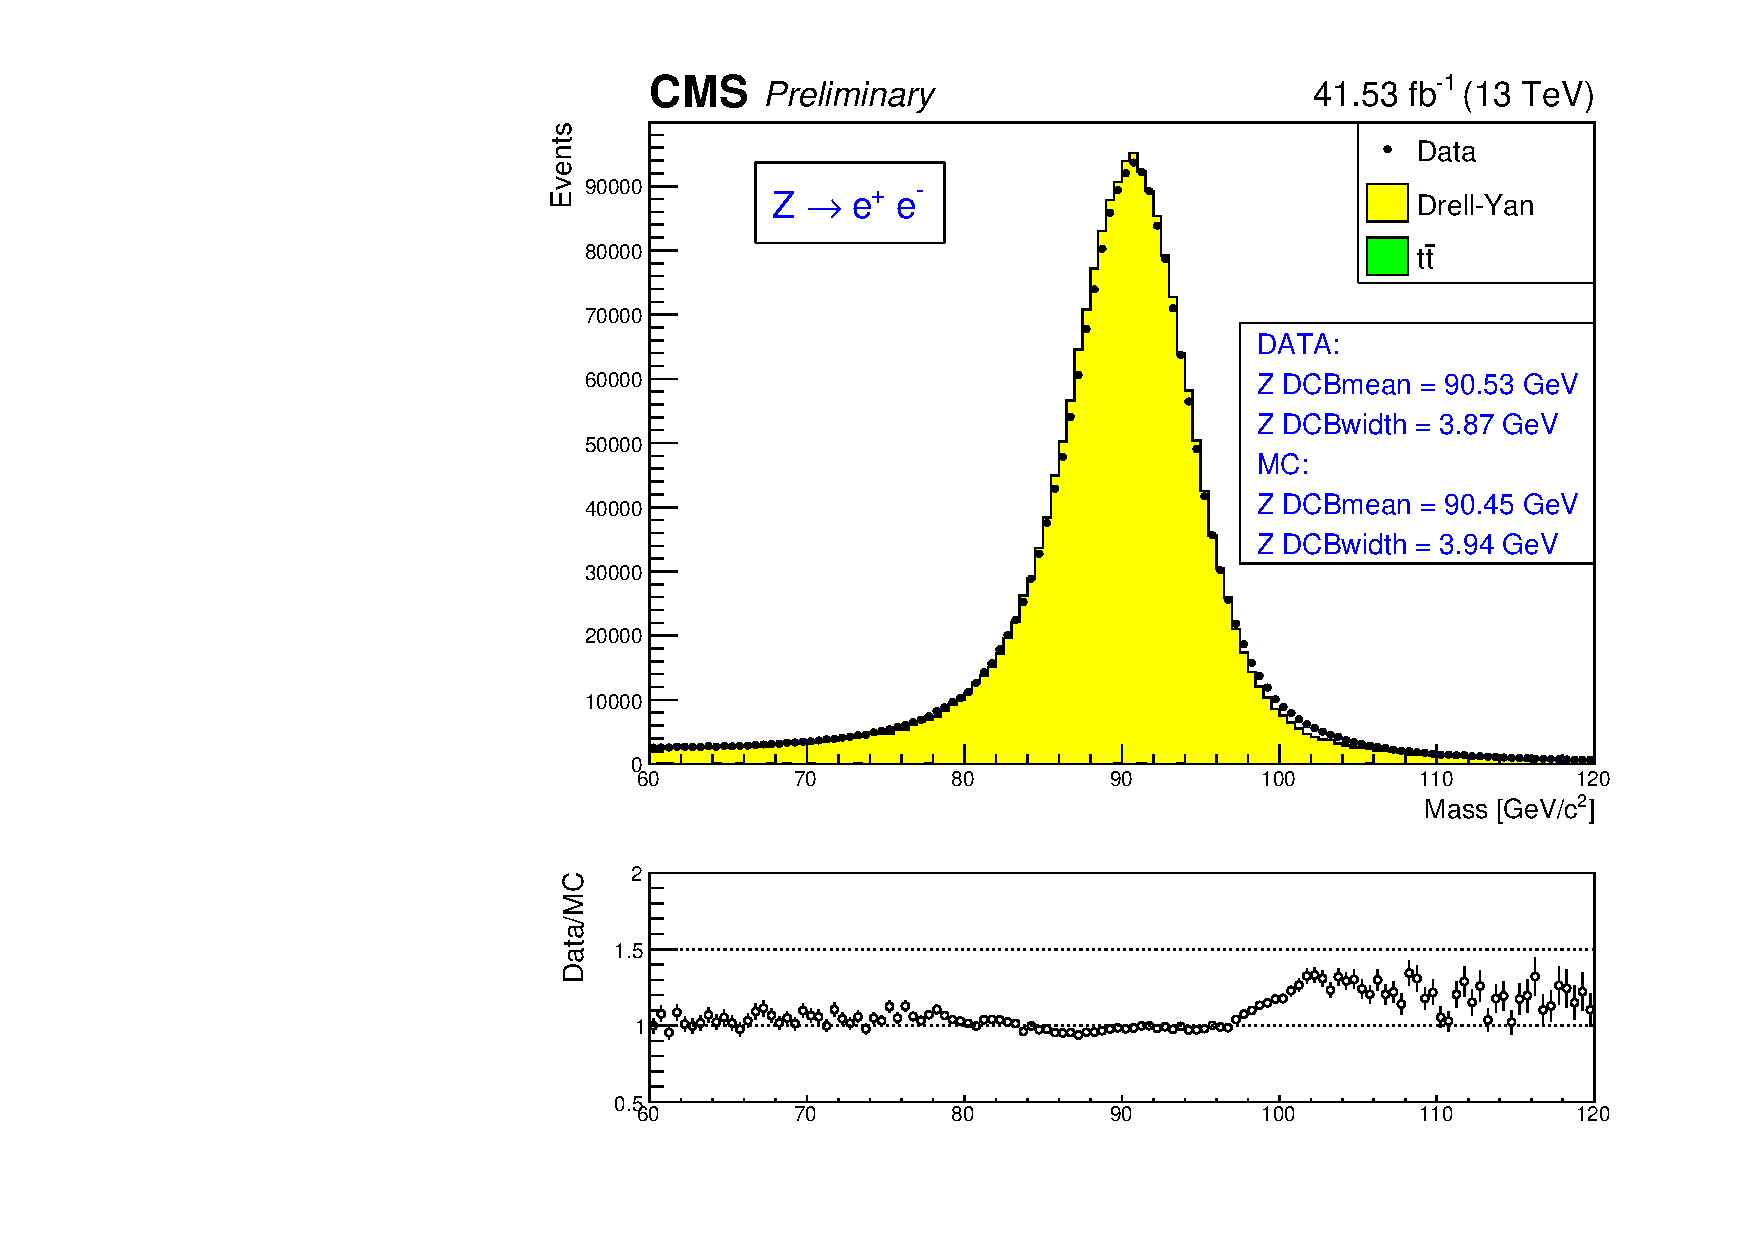
\includegraphics{Figures/Electrons/2017_ZMass_ele_EEEE.pdf}}} \\
%\end{center}
%\caption{
%(a): electron energy scale measured in the $Z\rightarrow \Pe \Pe$ control region for all electrons, for both electrons in the barrel (b), for one electron in the barrel, one in the endcaps (c) and for both electrons in the endcaps (d), for 2017 data.
%The results of the Crystall-ball fit are reported in the figures.
%%\textbf{FIXME: e-scale and smearing corrections NOT yet available and thus NOT yet applied} 
%}
%\label{fig:ele_energy_scaleB}
%\end{figure}
%
%\begin{figure}[!htb]
%\vspace*{0.3cm}
%\begin{center}
%\subfigure [] {\resizebox{8cm}{!}{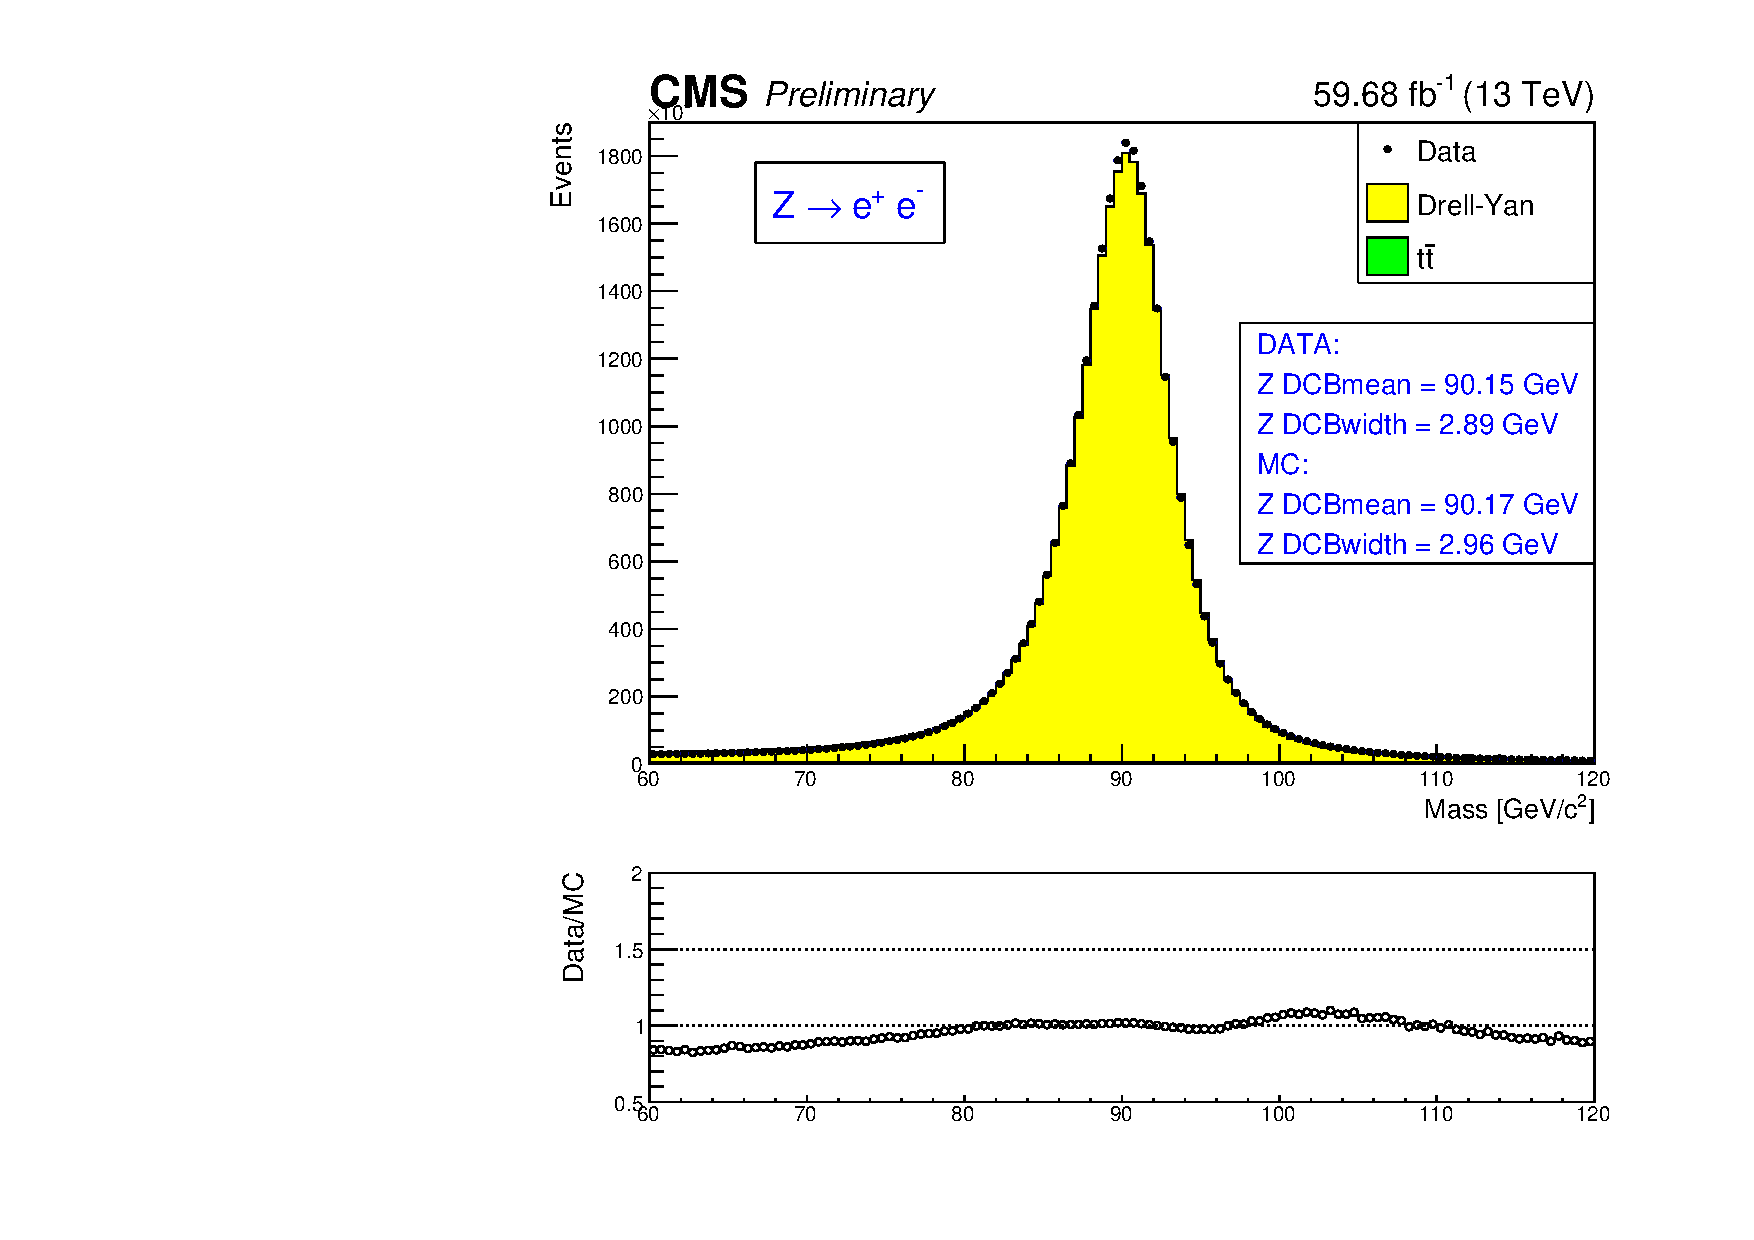
\includegraphics{Figures/Electrons/2018_ZMass_ele.pdf}}}
%\subfigure [] {\resizebox{8cm}{!}{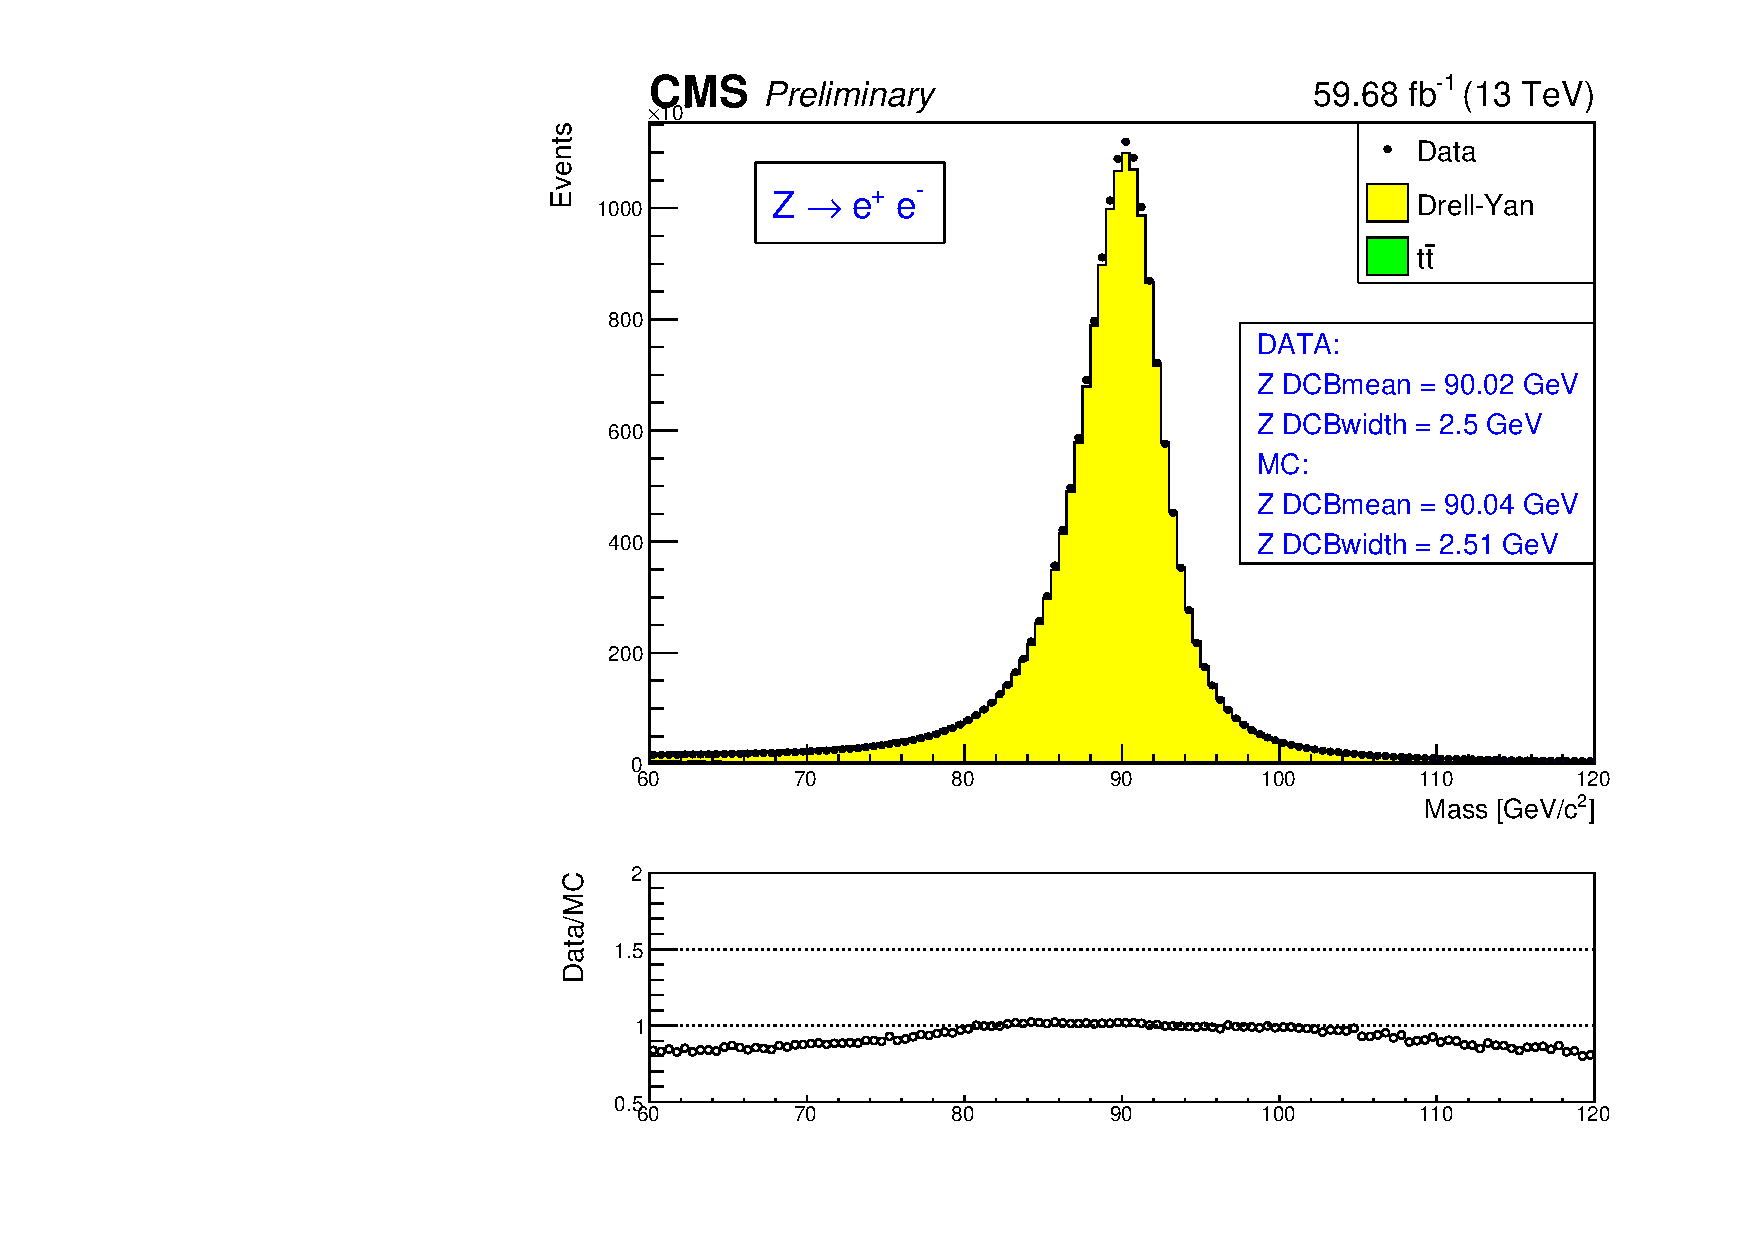
\includegraphics{Figures/Electrons/2018_ZMass_ele_EBEB.pdf}}} \\
%\subfigure [] {\resizebox{8cm}{!}{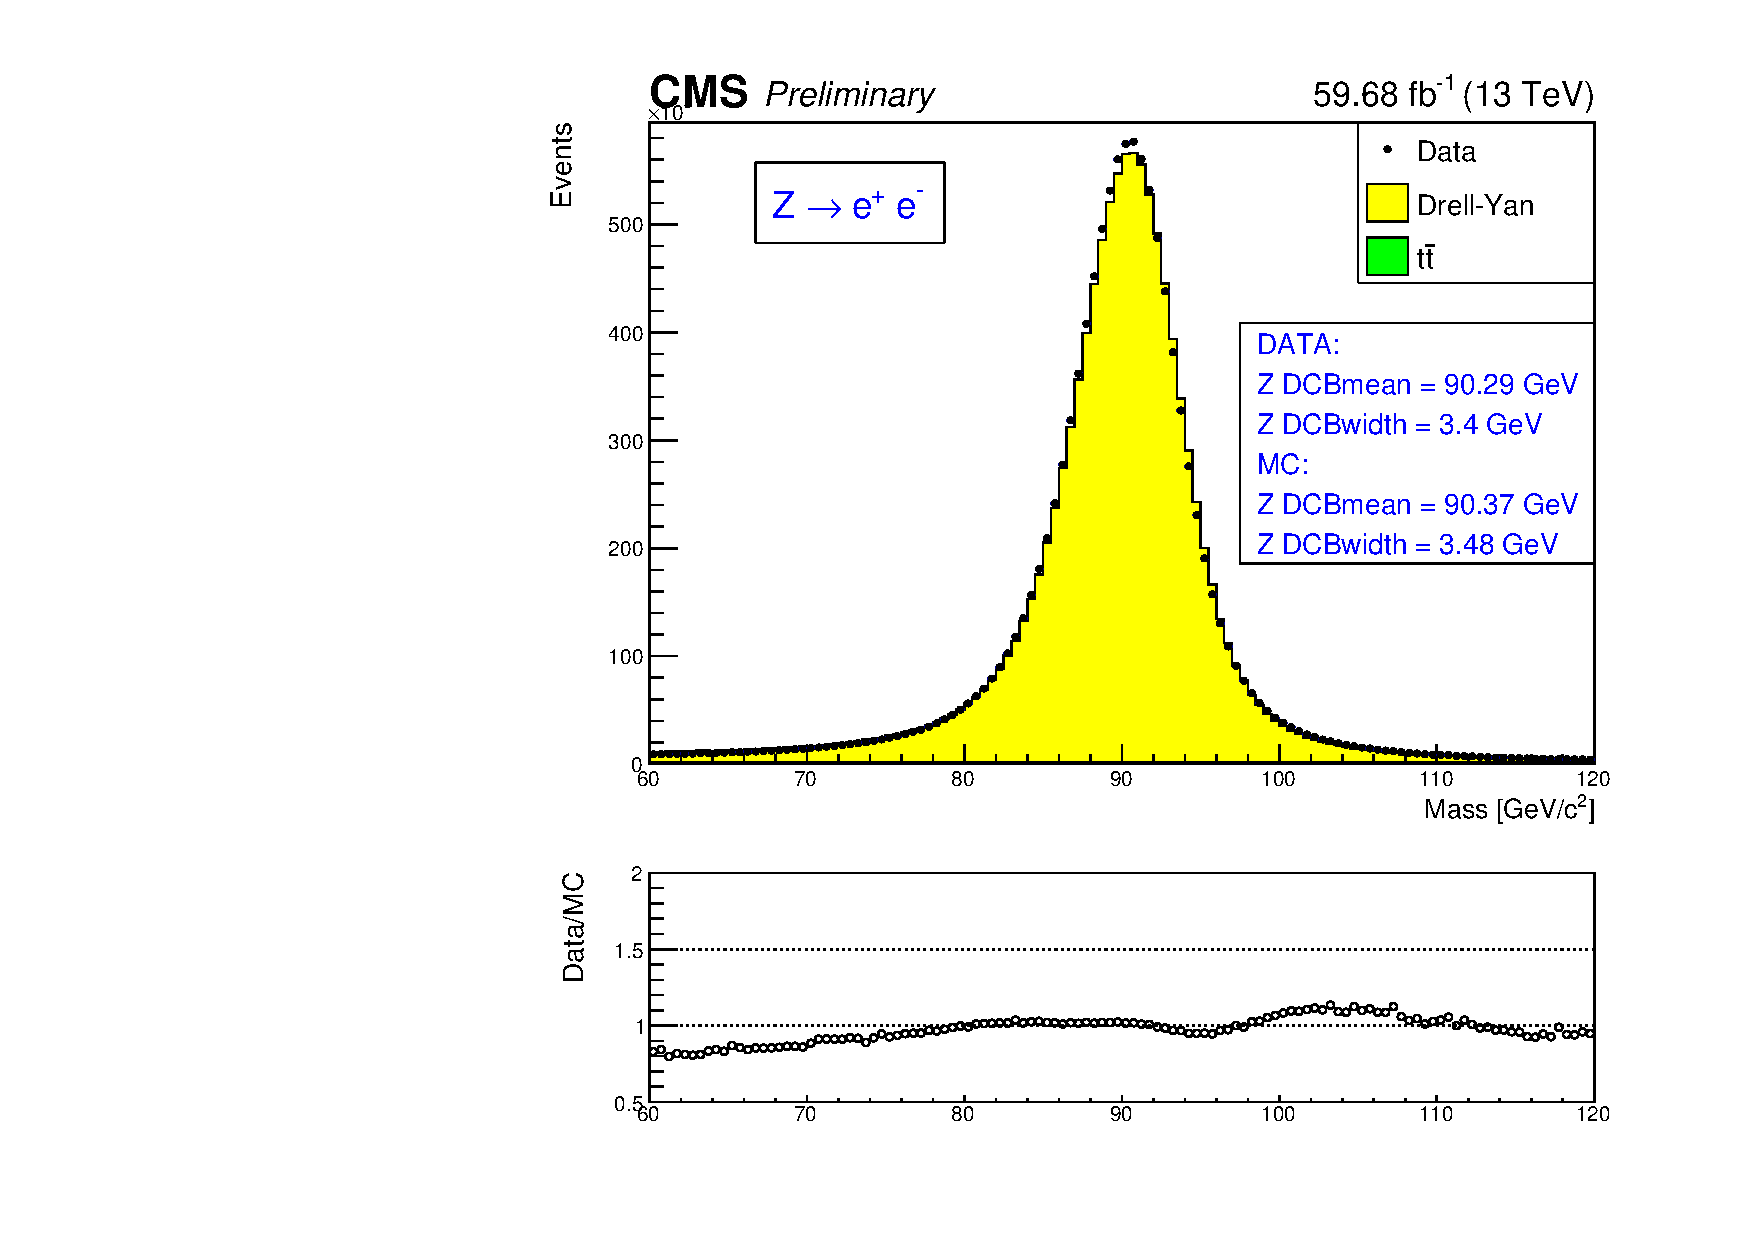
\includegraphics{Figures/Electrons/2018_ZMass_ele_EBEE.pdf}}}
%\subfigure [] {\resizebox{8cm}{!}{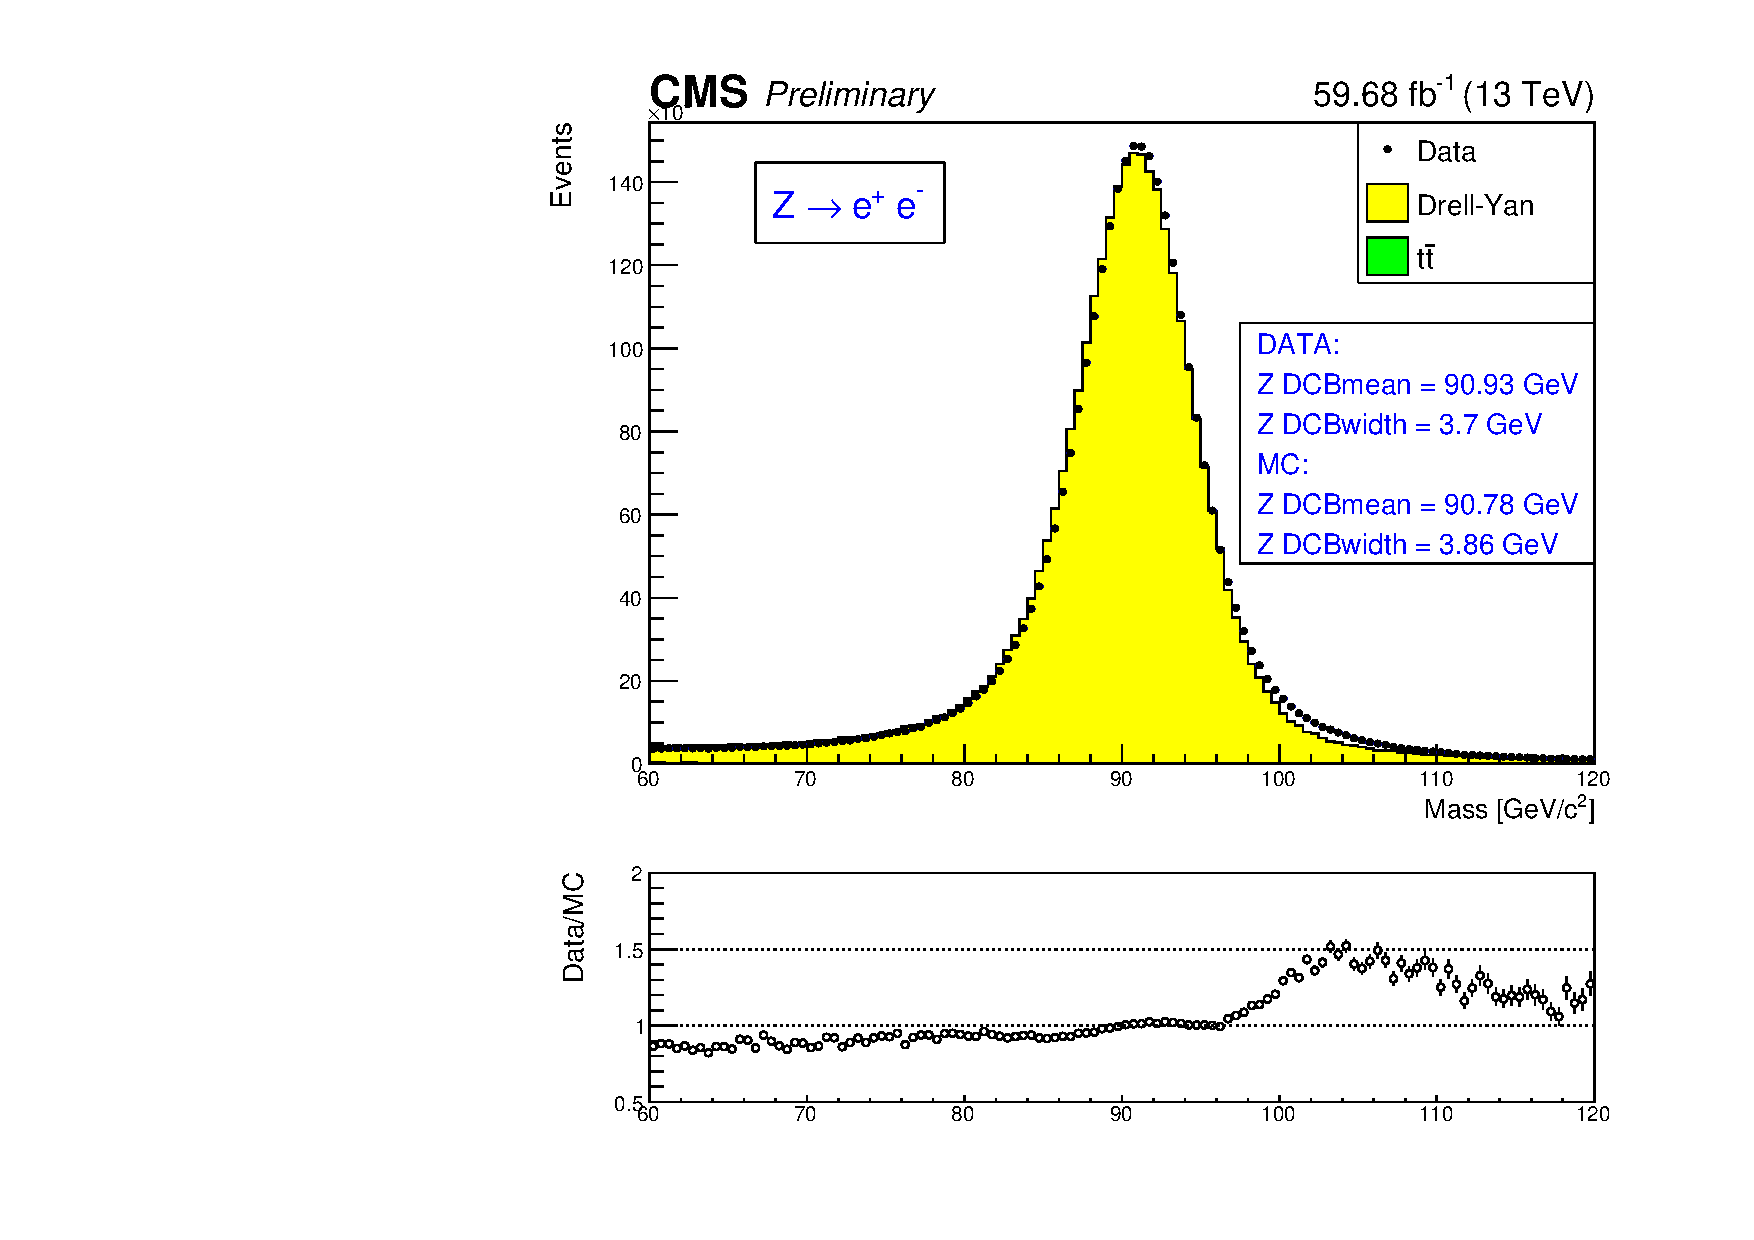
\includegraphics{Figures/Electrons/2018_ZMass_ele_EEEE.pdf}}} \\
%\end{center}
%\caption{
%(a): electron energy scale measured in the $Z\rightarrow \Pe \Pe$ control region for all electrons, for both electrons in the barrel (b), for one electron in the barrel, one in the endcaps (c) and for both electrons in the endcaps (d), for 2018 data.
%The results of the Crystall-ball fit are reported in the figures. 
%%\textbf{FIXME: e-scale and smearing corrections NOT yet available and thus NOT yet applied} 
%}
%\label{fig:ele_energy_scaleC}
%\end{figure}
%
%\clearpage
